\documentclass[12pt]{report}  
\usepackage{mathptmx}         
\parindent0pt  \parskip10pt             
\raggedright  
\usepackage{graphicx}                          

\title{\bf REAL TIME FACIAL EXPRESSION RECOGNITION }  
\author{ Name: Mahamat Nour Ali Mai\\
	Matric No: 1510455 \\ 
	[1cm]
	Name: Ilham Amka Fadillah \\
	Matric No: 1510455\\
	[1cm]
	Supervised by\\
	[1.5cm]
	Assoc. Prof. Dr Amelia Ritahani Ismail\\}  
             
\date{\today}                           

\begin{document}                        
\maketitle                              
\pagenumbering{roman}                   
\setcounter{page}{2}                    
\tableofcontents                        

\chapter{Background}               
\pagenumbering{arabic}                 
Face is the most distinctive and widely used key to
identity a person face. \texttt{Face} detection and facial feature extraction have attracted considerable attention in the advancement of human-machine interaction as it provides a natural and efficient way to communicate between humans and machines. The problem of \texttt{detecting} \texttt{faces} and \texttt{facial} parts in image sequences has become a popular area of research due to emerging applications in human-computer interface, surveillance systems, secure access control, video conferencing, financial transaction, forensic applications.

Computer or machine vision is a field in artificial intelligence that has become a great area of research due to its wide range of applications. From automated navigation of vehicles to medical imaging, all these applications require the computer to process, understand and analyses a scenario in order to make intelligent decisions.

With the power of computers today and the current breakthrough in technologies,
there are now various methods/algorithms that were developed to enable a
computer/machine to perform tasks such as face detection with emotion features. In this study, the focus will be on real time face detection with emotion features as our object of interest. 

Real time face detection with features have important roles in the security industry,
people demographic analysis, intelligent transportation system (ITS), classes attendance and work attendance on time.

\section{Objective}                 
To study on how face detection and real time facial expression tracking can be applied and used in real live world applications. To develop a model using Convolutional Neural Network (CNN) that will be use to detect face and facial expression. To test the model with images and videos to detect facial expressions. 

 
\section{Problem Statement}                 
The development of a reliable algorithm to perform face detection is still a challenge today. Despite the success of many systems and algorithm on face detection, many issues remain to be addressed. However, among those issue features face detection and real live face detection are some of the challenges faced today. 

 
\section{Project Scope}     
            
In this project, our attention will be on developing an algorithm to detect face features and real live time face detection with feature on videos. 

\section{Grant Chart}     

This grant chart will help us to visualize and view the tasks schedule over time.

\chapter{Literature Review}               
\pagenumbering{arabic} 
                
\section{Classification of Face detection Methods}                 
Generally there are many different types of approach used in face detection. In this approach we are going to use three approaches which are pre-processing, face detection, facial component detection, features extraction and classifier. the process of theses three approaches has shown in the figure1 below. 
\subsection{Pre-processing}

This is the first step of any image processing technique. In this stage we make the input image compatible for processing. The image may be taken under different conditions using different equipment. So the images that we get may not be in a standard form. The Input image may also be affected by various disturbances like noise, illumination variations, backgrounds etc.
\subsection{Face Detection}

Once the image is pre-processed our next aim is to remove all the unwanted back grounds and extract the face alone for further processing.
\subsection{Facial Component detection}

In this stage various Region of Interest are detected. The ROIs in Face detection are Eyes, eyebrows, nose, mouth/lips, ear, fore head etc.
\subsection{Features Extraction}

This is the most critical stage in facial expression recognition. the technique will be use to implement in this stage is critical as it's going to determine the efficiency of facial expression recognition.

\subsection{Classification}
In this stage the classifier classifies the features that are
extracted from the face images to the respective facial expression
classes.

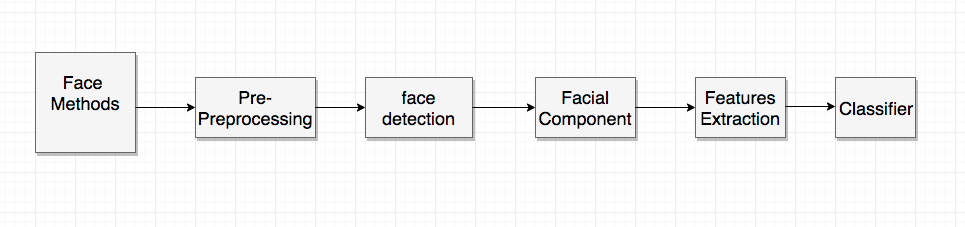
\includegraphics[width = 15cm, height = 9cm ]{figure1.png}
Figure 1: Classification of face detections

 
\end{document}                         
